%%%%%%%%%%%%%%%%%%%%%%%%%%%%%%%%%%%%%%%%%%%%%%%%%%%%%%%%%%%%%%%%%%%%%%
%
\section{Figures and Tables}
%
%%%%%%%%%%%%%%%%%%%%%%%%%%%%%%%%%%%%%%%%%%%%%%%%%%%%%%%%%%%%%%%%%%%%%%

This section defines the
special commands that are available only at the IVT environment.
Those special commands
react on different layouts defined in the environment,
thus making it convenient to switch between paper layouts.

%%%%%%%%%%%%%%%%%%%%%%%%%%%%%%%%%%%%%%%%%%%%%%%%%%%%%%%%%%%%%%%%%%%%%%
\subsection{Figures} \label{sec:compStructs-Figures}
%%%%%%%%%%%%%%%%%%%%%%%%%%%%%%%%%%%%%%%%%%%%%%%%%%%%%%%%%%%%%%%%%%%%%%

There are three commands for including Figures. One for a single Figure
and one for a Multi-Figure. The position of the Figure is chosen by
\LaTeX,
but a hint can be provided.

\subsubsection{Single Figures}

\label{sec:compStructs-Figures-SingleFigures}

A single figure as shown in \cref{fig:labelOfTheSingleFigure}
has the following construct:

\textbackslash{}begin[placement]\{figure\} as in normal latex 

The placement modifier 
specifies where the figure appears in the final document.
It can be ``tp'', ``htp'' or ``hp'';
``t'' means ``at the top of this or a following page'',
``h'' means ``at the place where the command appears'',
and ``p'' means ``on a separate page''.
If you leave out this parameter (including the square brackets),
``tp'' is the default.
Usually a figure will appear on the next suitable location
after it has been declared.
The placement on a separate page will be used as a last resort
if the figure does not fit anywhere else, even if you do not include it.

With \textbackslash{}ivtsource\{text\} you can add a source. If you do not want
to add a source, just leave it empty. If not, ``Source: '' or
``Quelle: '' will be added followed by your text.


%---------------------------------------------------------------------
\begin{figure}%
\caption{Single Figure: Here you can add the long Caption of the Figure.}%
\label{fig:labelOfTheSingleFigure}%
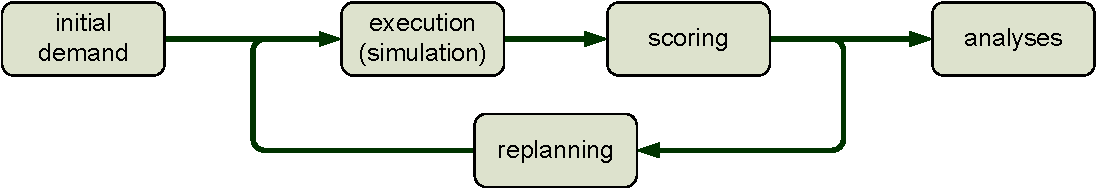
\includegraphics[width=1.0\textwidth]{figures/MATSimLoop}%
\ivtsource{Christoph Dobler}
\ivthline
\end{figure}

%%%%%%%%%%%%%%%%%%%%%%%%%%%%%%%%%%%%%%%%%%%%%%%%%%%%%%%%%%%%%%%%%%%%%%
\subsection{Tables} \label{sec:compStructs-Tables}
%%%%%%%%%%%%%%%%%%%%%%%%%%%%%%%%%%%%%%%%%%%%%%%%%%%%%%%%%%%%%%%%%%%%%%

A table has the same structure as the single Figure (see above). But
instead of including a graphic in item~4 you add the ``tabular''
construct.
Unfortunately it is not that easy to understand and edit such a table. One has
to get used to it. 
However, quite a few tools can help converting the data
to the \LaTeX{} format,
see \url{http://tex.stackexchange.com/q/49414/8057}
for an overview.

If you do not like it you can still add the table
as a graphic (with the ``\textbackslash{}includegraphics'') command.
But you still need
to use the ``\textbackslash{}createtable'' command,
otherwise your table will appear
in the list of figures instead of the list of tables.
\Cref{tab:labelOfTheTable} shows an example of a table.

%---------------------------------------------------------------------
\begin{table}[!ht]
\caption{A Tables  Caption}
\label{tab:labelOfTheTable}%

\begin{tabular}[c]{lr@{.}lcr@{.}l}
    \toprule
    Bias / Error     & \multicolumn{2}{c}{Routes Only} &
\multicolumn{3}{c}{Times and Routes} \\
    \midrule
    Mean Abs. Bias:  & $+$331&40                        && $+$306&32  
                         \\
    Mean Rel. Bias:  &  $+$19&62\%                      &&  $+$25&27\%
                         \\
    \midrule
    Mean Abs. Error: &    533&55                        &&    503&77  
                         \\
    Mean Rel. Error: &     37&50\%                      &&     35&38\%
                         \\
    \bottomrule
  \end{tabular}

\ivtsource{my source}
\ivthline
\end{table}
%---------------------------------------------------------------------

\begin{figure}
\centering

\caption{Standardisierte Verteilungsfunktionen der Kurzdistanzen (MZ).}
\label{fig:mz-fit}

\begin{subfigure}{0.49\textwidth}
    \centering
    \caption{Verteilungsfunktion der GTD <100km.}
    \label{subfig:mz-fit-met-1}
    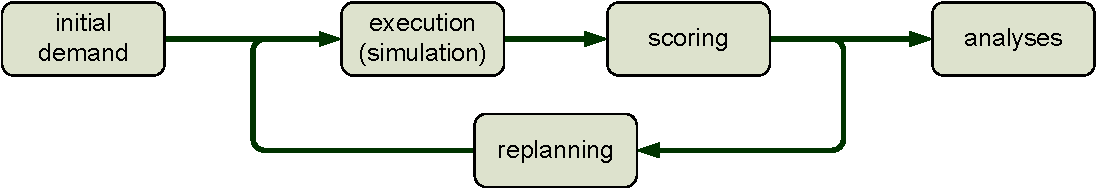
\includegraphics[width=0.8\textwidth]{figures/MATSimLoop.pdf}
\end{subfigure}
\begin{subfigure}[]{0.49\textwidth}
    \centering
    \caption{Verteilungsfunktion der Wege <100km.}
    \label{subfig:mz-fit-met-2}
    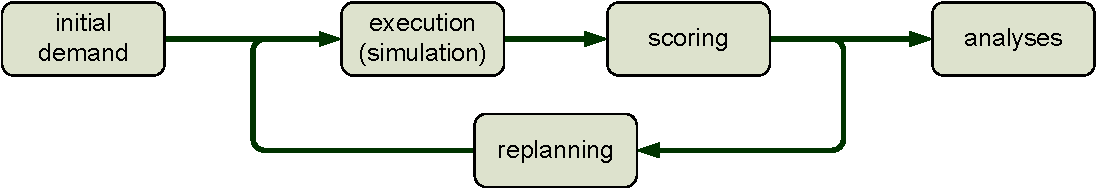
\includegraphics[width=0.8\textwidth]{figures/MATSimLoop.pdf}
\end{subfigure}

\ivtsource{my source}

\ivthline
\end{figure}
